% !TEX spellcheck=en_US
\documentclass[a4paper]{article}
\usepackage[american]{babel}
\usepackage[T1]{fontenc}
\usepackage[utf8]{inputenc}
\usepackage[activate={true,nocompatibility},final,tracking=true,kerning=true,spacing=true,factor=1100,stretch=10,shrink=10]{microtype}
\usepackage{graphicx}
\usepackage[table,dvipsnames]{xcolor}
\usepackage{caption}
\usepackage{subcaption}
\usepackage{csquotes}
\usepackage{hyperref}
\usepackage[super]{nth}
\usepackage{amsmath}
\usepackage{amssymb}
\usepackage{amsthm}
\usepackage{mathtools}
\usepackage{mathmacros/mathmacros}
\usepackage{tcolorbox}
\usepackage{circuitikz}
\usepackage{tikz}
\usepackage{pgf}
\usepackage{pgfplots}
\usepackage[acronym]{glossaries}
\usepackage[backend=biber,style=phys]{biblatex}

% environments
\newtheorem{lemma}{Lemma}
\newtheorem{thm}{Theorem}
\newtheorem{crl}{Corollary}
\newtheorem{definition}{Definition}
\theoremstyle{remark}
\newtheorem{exm}{Example}
\theoremstyle{remark}
\newtheorem{rem}{Remark}

% misc macros
\newcommand*{\pref}[2]{#1 (\ref{#2})}
\definecolor{lightgray}{rgb}{0.9725,0.9725,0.9725}

% microtype
\SetTracking{encoding={*}, shape=sc}{0}

% pgfplots
\pgfplotsset{compat=newest}

\addbibresource{bibliography.bib}

\makenoidxglossaries
\newacronym{dne}{DNE}{does not exist}
\newacronym{wlog}{WLOG}{without loss of generality}

\begin{document}

\begin{titlepage}
    \centering
    {\scshape\Huge \bfseries{Advanced Systems} \par}
    \par\vspace{1cm}
    
\includegraphics[width=0.45\textwidth]{images/logo.png}\par
    \vspace{3cm}
    {\huge\bfseries Lecture Notes \par}
    \vspace{1cm}
    {\LARGE\itshape Mazawa Shinonome \par}
    \vspace{1cm}
    {\large\today\par}
    \vfill
    \begin{abstract}
        This document is a compilation of lecture notes for intermediate mathematics.
        It is intended to serve as a study guide for members of the Advanced System
        organization.
    \end{abstract}
\end{titlepage}

\newpage

\microtypesetup{protrusion=false}
\clearpage
\printnoidxglossaries
\newpage
\tableofcontents
\microtypesetup{protrusion=false}

\newpage

% === Begin Section Includes ===

\section{Acknowledgements}

TODO


\section{Introduction}

\begin{flushleft}
	The Advanced System organization is an open-source software community who's main
	purpose it is to develop modern and user-friendly utility programs. In order to
	develop advanced applications, the study of mathematics is of particular interests:
	It lays the groundwork for many other fields of studies such as physics or computer
	science.
\end{flushleft}

\begin{flushleft}
	While this document has been drafted with the best intents and purposes, there
	is no warranty on the correctness of its content. You can find the source code
	on \url{www.github.com/Advanced-Systems/lecture-notes} to compile a new PDF
	file from scratch using the most recent version of this document or raise an
	issue to report mistakes under the issues tab of GitHub.
\end{flushleft}


\section{Single Variable Calculus}\label{sec-single-var-calc}

TODO: Add descriptions


\section{Logic}\label{sec-logic}

% ==============================================================================
% ==============================================================================
% ==============================================================================

\subsection{Truth Tables}\label{subsec-truth-table}

Propositional logic is a formal mathematical framework that encodes the truth value
of one or more propositions. A proposition is a statement that, by itself, is either
true or false. These propositions can be combined with binary operations to determine
the truth value of a statement expressed in the vernacular. While every proposition
is a statement, not every statement is a valid proposition.

\begin{enumerate}
    \item Questions are invalid propositions.
    \item Statements where the intention is unclear or ambiguous don't qualify as propositions, either.
\end{enumerate}

In practice, the variables \(A,B,C,\dots\) are often used to denote propositions.
Therefore, they are also sometimes referred to as \emph{propositional variables}
that can take on one of two possible values: \(T\) (true) or \(F\) (false). In
computer science, \(1\) (true) or \(0\) (false) are commonly used instead. It is
worth adding that many programming languages interpret any number \(n\neq0\) as
true\footnote{Take Python or C++ as prominent examples for this behavior.}. While
propositional logic has its place, inference systems are used in formal reasoning
instead, though this topic is beyond the scope of this subsection.

\begin{definition}\label{def-axiom}
    An axiom is a statement that is taken to be true and is confined within the
    system of logic they define. They establish the premise of reasoning and cannot
    be formally proved.
\end{definition}

There are five important axioms from which one can obtain a series of useful logical
statements that will later be used to formulate mathematical sound proofs. In order
to make this material more accessible, each axiom will be prefaced by a quote written
in the vernacular that accurately reflects the statement in question.

\begin{displayquote}
    ``\emph{It takes courage and strength to be empathetic.}''
    --- Jacinda Ardern\footnote{New Zealand politician who has been serving as the
    40th prime minister of New Zealand and leader of the Labour Party since 2017.}
\end{displayquote}

In this example, a person is said to be empathetic (\(C\)) if one is both
courageous (\(A\)) \emph{and} strong in character (\(B\)).

\begin{table}[hbt!]
    \centering
    \rowcolors{1}{}{lightgray}
    \begin{tabular}{*{6}{c}}
        $(A$ & $\land$ & $B)$ & $\rightarrow$ & $C$ \\
           T &         & T    &               & T   \\
           T &         & F    &               & T   \\
           F &         & T    &               & F   \\
           F &         & F    &               & F   \\
    \end{tabular}
    \caption{Conjunction}\label{table-conjunction}
\end{table}

\begin{displayquote}
    ``\emph{So much of life is not about whether you're good or bad, or right or
    wrong, or can afford or not afford -- it's about timing.}''
    -- Adrian Anthony Gill\footnote{Scottish writer and critic.}
\end{displayquote}

In natural languages, a distinction is often drawn implicitly between inclusive
and exclusive disjunctions. See \pref{table}{table-disjunction} as an example of
the inclusive disjunction (\emph{or}). The truth table for the exclusive disjunction
(\emph{xor}) will be introduced later in \pref{subsection}{subsec-circuit-representation}.

\begin{table}[hbt!]
    \centering
    \rowcolors{1}{}{lightgray}
    \begin{tabular}{*{6}{c}}
        $(A$ & $\lor$ & $B)$ & $\rightarrow$ & $C$ \\
           T &        & T    &               & T   \\
           T &        & F    &               & T   \\
           F &        & T    &               & T   \\
           F &        & F    &               & F   \\
    \end{tabular}
    \caption{Disjunction}\label{table-disjunction}
\end{table}

\begin{displayquote}
    ``\emph{'Awkward' implies both solidarity and implication. Nobody is exempt.}''
    -- Elif Batuman\footnote{American author, academic, and journalist.}
\end{displayquote}

One interesting thing to note about \pref{table}{table-subjunction} is that it is
possible to arrive to true statements even if the premise or assumption turned out
to be incorrect, an important implication of this being that there are no valuable
insights to be gained from a false premise. Therefore, it is of utmost importance
in logical reasoning to verify that the starting arguments have a positively affirmative
truth value.

\begin{table}[hbt!]
    \centering
    \rowcolors{1}{}{lightgray}
    \begin{tabular}{*{6}{c}}
        $(A$ & $\Rightarrow$ & $B)$ & $\rightarrow$ & $C$ \\
           T &               & T    &               & T   \\
           T &               & F    &               & F   \\
           F &               & T    &               & T   \\
           F &               & F    &               & T   \\
    \end{tabular}
    \caption{Subjunction}\label{table-subjunction}
\end{table}

\begin{displayquote}
    ``\emph{One man is equivalent to all Creation. One man is a World in miniature.}''
    -- Albert Pike\footnote{American author, poet, orator, editor, lawyer, jurist,
    and prominent member of the Freemasons}
\end{displayquote}

Logically equivalent statements share the same truth value across all occurring
propositional variables. They become important later in ring proofs where multiple
distinct propositions implicate each other in all directions.

\begin{table}[hbt!]
    \centering
    \rowcolors{1}{}{lightgray}
    \begin{tabular}{*{6}{c}}
        $(A$ & $\Leftrightarrow$ & $B)$ & $\rightarrow$ & $C$ \\
           T &                   & T    &               & T   \\
           T &                   & F    &               & F   \\
           F &                   & T    &               & F   \\
           F &                   & F    &               & T   \\
    \end{tabular}
    \caption{Bisubjunction}\label{table-bisubjunction}
\end{table}

\begin{exm}\label{exm-logical-equivalent}
    It is left to the reader as an exercise to use a truth table to verify the
    following proposition:
    \begin{equation}
        \left((A \Rightarrow B) \land (B \Rightarrow A)\right) \Leftrightarrow (A \Leftrightarrow B)
    \end{equation}
\end{exm}

\begin{displayquote}
    ``\emph{No worse fate can befall a young man or woman than becoming prematurely
    entrenched in prudence and negation.}''
    -- Knut Hamsun\footnote{Norwegian writer and Nobel Prize winner in Literature
    in 1920.}
\end{displayquote}

Negation is one of the simplest unary operations in that it inverts the truth
value of a propositional variable.

\begin{table}[hbt!]
    \centering
    \rowcolors{1}{}{lightgray}
    \begin{tabular}{*{6}{c}}
        $(\neg B)$ & $\rightarrow$ & $C$ \\
                 T &               & F   \\
                 F &               & T   \\
    \end{tabular}
    \caption{Negation}\label{table-negation}
\end{table}

% ==============================================================================
% ==============================================================================
% ==============================================================================

\subsection{Circuit Representation of Logical Operations}\label{subsec-circuit-representation}

Truth tables are very useful in determining the nature of logic gates.
In \pref{table}{subsec-truth-table} find defined the axioms which build the basis for
this section. Take \texttt{XOR}, for instance: this logic gate evaluates to $1$
if and only if one of both poles receives $1$ as an input as opposed to \texttt{OR}
which also accepts two positive-valued states favorably.

\begin{table}[hbt!]
    \centering
    \rowcolors{1}{}{lightgray}
    \begin{tabular}{*{6}{c}}
        $A$ & $B$ & $A\texttt{ OR }B$ & $A\texttt{ AND }B$ & $A\texttt{ NAND }B$ & $(A\texttt{ OR }B)\texttt{ AND }(A\texttt{ NAND }B)$ \\
          1 & 1   & 1                 & 1                  & 0                   & 0                                                    \\
          1 & 0   & 1                 & 0                  & 1                   & 1                                                    \\
          0 & 1   & 1                 & 0                  & 1                   & 1                                                    \\
          0 & 0   & 0                 & 0                  & 1                   & 0                                                    \\
    \end{tabular}
    \caption{\texttt{XOR} Truth Table}\label{truth-table-xor}
\end{table}

Based on this truth table it is possible to implement a logic gate that replicates
a \texttt{XOR} gate in the following way:

\begin{figure}[hbt!]
    \centering
    \begin{circuitikz}
        % gates
        \node[or port,draw] at (0,2) (or) {};
        \node[nand port,draw] at (0,0) (nand) {};
        \node[and port,draw] at (2,1) (and) {};
        % inputs
        \node at ($(or.in 1) + (-1,0)$) (A) {$A$};
        \node at ($(nand.in 2) + (-1,0)$) (B) {$B$};
        % wires
        \draw (A) -- (or.in 1);
        \draw (A) -- (nand.in 1);
        \draw (B) -- (or.in 2);
        \draw (B) -- (nand.in 2);
        \draw (or.out) -- (and.in 1);
        \draw (nand.out) -- (and.in 2);
        \draw (and.out) -- ($(and.out) + (0.5,0)$) node[anchor=west] (Q) {$Q$};
    \end{circuitikz}
    \caption{Circuit of an \texttt{XOR} gate}\label{circuit-xor-gate}
\end{figure}

A half adder is a circuit that adds two binary numbers, each one bit in size.
The result $S$ is also represented by a one bit value, so in case of 
$1_2+1_2=(10)_2$ the second digit must be carried over in $C$ (hence the name 
\textit{carrier}) in order to be preserved for future operations.

\begin{figure}[hbt!]
    \centering
    \begin{circuitikz}
        % xor gate
        \node[xor port,draw] at (0,2) (xor) {};
        \draw (xor.in 1) -- ($(xor.in 1) + (-0.75,0)$) node[anchor=east] (A) {$A$};
        \draw (xor.in 2) -- ($(xor.in 2) + (-0.75,0)$) node[anchor=east] (B) {$B$};
        \draw (xor.out) -- ($(xor.out) + (0.75,0)$) node[anchor=west] (S) {$S$};
        % and gate   
        \node[and port,draw] at (0,0) (and) {};
        \draw (xor.in 1) -- (and.in 1);
        \draw ($(xor.in 2) + (-0.25,0)$) -- ($(and.in 2) + (-0.25,0)$) -- (and.in 2);
        \draw (and.out) -- ($(and.out) + (0.75,0)$) node[anchor=west] (C) {$C$};        
    \end{circuitikz}
    \caption{Circuit of an half adder}\label{circuit-half-adder}
\end{figure}

\begin{table}[hbt!]
    \centering
    \rowcolors{1}{}{lightgray}
    \begin{tabular}{*{4}{c}}
        $A$ & $B$ & $S$ & $C$ \\
          1 & 1   & 0  & 1    \\
          1 & 0   & 1  & 0    \\
          0 & 1   & 1  & 0    \\
          0 & 0   & 0  & 0    \\
    \end{tabular}
    \caption{Half Adder Truth Table}\label{truth-table-half-adder}
\end{table}

As opposed to an half adder, a full adder takes one more input (a so-called \texttt{carry in})
and two outputs, \textit{i.e.} \texttt{carry out} and \texttt{sum}. To build a
more sophisticated adder, chain half adders in a way that allows the result of
the previous sum to be carried over as \texttt{cin} to the next half adder.

\begin{figure}[hbt!]
    \centering
    \begin{circuitikz}
        % gates
        \node[xor port,draw,anchor=center] at (0,4) (xor1) {D};
        \node[xor port,draw] at (2,4) (xor2) {};
        \node[and port,draw] at (2,2) (and1) {E};
        \node[and port,draw] at (2,0) (and2) {F};
        \node[or port,draw] at (4,1) (or) {};
        % inputs
        \node at ($(xor1.in 1) + (-1,0)$) (A) {$A$};
        \node at ($(xor1.in 2) + (-1,0)$) (B) {$B$};
        \node at ($(A) + (0,-1.5)$) (C) {$C_{in}$};
        % wires
        \draw (A) -- (xor1.in 1);
        \draw (B) -- (xor1.in 2);
        \draw (xor1.out) -- (xor2.in 1);
        \draw (C) -- (xor2.in 2);
        \draw (C) -- (and1.in 1);
        \draw (xor1.out) -- ($(and1.in 2)-(0.5,0)$) -- (and1.in 2);
        \draw ($(A)+(0.75,0)$) -- ($(A)+(0.75,-4.56)$) -- (and2.in 2);
        \draw ($(B)+(1,0)$) -- ($(B)+(1,-3.425)$) -- (and2.in 1);
        \draw (and1.out) -- (or.in 1);
        \draw (and2.out) -- (or.in 2);
        \draw (xor2.out) -- ($(xor2.out) + (0.5,0)$) node[anchor=west] (S) {$S$};
        \draw (or.out) -- ($(or.out) + (0.5,0)$) node[anchor=west] (Q) {$C_{out}$};
    \end{circuitikz}
    \caption{Circuit of an full adder}\label{circuit-full-adder:1}
\end{figure}

Circuit \pref{figure}{circuit-full-adder:1} introduced three additional truth values 
to make the truth \pref{table}{truth-table-full-adder} for the full adder easier
to read\footnote{Note that $S:\Leftrightarrow D\texttt{ XOR } C_{in}$ and 
$C_{out} :\Leftrightarrow E\texttt{ OR }F$}. It is helpful to think of gate $D$
and gate $F$ as the first half adder.

\begin{table}[hbt!]
    \centering
    \rowcolors{1}{}{lightgray}
    \begin{tabular}{*{8}{c}}
        $A$ & $B$ & $C_{in}$ & $A\texttt{ XOR }B$ & $D\texttt{ XOR }C_{in}$ & $D\texttt{ AND }C_{in}$ & $F$ & $E\texttt{ OR }F$ \\
          1 & 1   & 1        & 0                  & 1                       & 0                       & 1   & 1                 \\
          1 & 1   & 0        & 0                  & 0                       & 0                       & 1   & 1                 \\
          1 & 0   & 1        & 1                  & 0                       & 1                       & 0   & 1                 \\
          0 & 1   & 1        & 1                  & 0                       & 1                       & 0   & 1                 \\
          1 & 0   & 0        & 1                  & 1                       & 0                       & 0   & 0                 \\
          0 & 1   & 0        & 1                  & 1                       & 0                       & 0   & 0                 \\
          0 & 0   & 1        & 0                  & 1                       & 0                       & 0   & 0                 \\
          0 & 0   & 0        & 0                  & 0                       & 0                       & 0   & 0                 \\
    \end{tabular}
    \caption{Full Adder Truth Table}\label{truth-table-full-adder}
\end{table}


\subsection{Sets}\label{subsec-sets}

% ==============================================================================
% ==============================================================================
% ==============================================================================

TODO: Add description

\subsubsection{Indicator Functions}\label{subsubsec-indicator-functions}

\begin{definition}\label{def-indicator-function}
	Let $X$ be a set. For each subset $A \subseteq X$ there is defined the
	indicator function\footnote{Sometimes, the term characteristic function is
		used to describe the function that indicates membership in a set in other
		fields of mathematics. The term indicator function is more prominently used
		in probability theory.} $\chi_A:X\rightarrow \{0,1\}$ of the set $A$ as
	\begin{equation}
		\chi_A(x) = \begin{cases}
			1,\;\text{ if } x \in A \\
			0,\;\text{ if } x \notin A
		\end{cases}
	\end{equation}
	We will write $\chi_A$ instead of $\chi_A(x)$ if the parameter
	$x$ is unambiguous.
\end{definition}

\begin{thm}\label{thm-complement-indicator-function}
	Let $\chi_A$ be an indicator function. Then the complement of $A$ (i.e.
	$\overline{A} \defines A^C$) is
	\begin{equation*}
		\chi_{\overline{A}} = 1 - \chi_A
	\end{equation*}
\end{thm}

\begin{proof}
	Of \pref{theorem}{thm-complement-indicator-function}.
	\begin{align*}
		\chi_{\overline{A}}(x) & = \begin{cases}
			1,\;\text{ if } \neg(x \in A) \\
			0,\;\text{ if } \neg(x \notin A)
		\end{cases}    \\
		                       & = \begin{cases}
			1-0,\;\text{ if } x \notin A \\
			1-1,\;\text{ if } x \in A
		\end{cases}    \\
		                       & =1 - \begin{cases}
			0,\;\text{ if } x \notin A \\
			1,\;\text{ if } x \in A
		\end{cases} \\
		                       & = 1 - \chi_A(x)
	\end{align*}
\end{proof}

\begin{thm}\label{thm-set-cardinality-indicator-function}
	Let $\chi_A$ be an indicator function with $A$ as a finite set. Then,
	\begin{equation*}
		\abs{A} = \sum_{x \in X} \chi_A(x)
	\end{equation*}
\end{thm}

\begin{proof}
	Of theorem (\ref{thm-set-cardinality-indicator-function}).
	\begin{align*}
		\abs{A} & =\sum_{x\in A}\underbrace{\chi_A(x)}_{1}                                   \\
		        & =\sum_{x\in A}\chi_A(x)+\sum_{x\in X\setminus A}\underbrace{\chi_A(x)}_{0} \\
		        & =\sum_{x\in (A\cup (X\setminus A))}\chi_A(x)                               \\
		        & \overset{(\star)}{=}\sum_{x\in X}\chi_A(x).
	\end{align*}
	since
	\begin{equation*}
		(\star) :\Leftrightarrow A\cup(X\setminus A)=(A\cup X)\setminus(A\setminus A)=X\setminus \emptyset=X
	\end{equation*}
\end{proof}

\begin{thm}\label{thm-cap-indicator-function}
	Let $\chi_A,\chi_B$ be indicator functions. Then:
	\begin{equation*}
		\chi_{A \cap B} = \chi_A\chi_B
	\end{equation*}
\end{thm}

\begin{proof}
	Of \pref{theorem}{thm-cap-indicator-function}.
	\begin{align*}
		\chi_{A \cap B} & = \begin{cases}
			1\;\text{ if } x \in (A \cap B) \\
			0\;\text{ if } x \notin (A \cap B)
		\end{cases}                                                     \\
		                & = \begin{cases}
			1\;\text{ if } x \in A \land x \in B \\
			0\;\text{ if } x \notin A \land x \notin B
		\end{cases}                                                     \\
		                & = \left(\begin{cases}
				1\;\text{ if } x \in A \\
				0\;\text{ if } x \notin A
			\end{cases}\right)\left(\begin{cases}
				1\;\text{ if } x \in B \\
				0\;\text{ if } x \notin B
			\end{cases}\right) \\
		                & = \chi_A\chi_B
	\end{align*}
\end{proof}

\begin{thm}\label{thm-cup-indicator-function}
	Let $\chi_A,\chi_B$ be indicator functions. Then:
	\begin{equation*}
		\chi_{A \cup B} = \chi_A + \chi_B - \chi_A\chi_B
	\end{equation*}
\end{thm}

\begin{proof}
	Of \pref{theorem}{thm-cup-indicator-function}.
	By using the fact that $\overline{\overline{A}}=A$ in combination with
	\pref{theorem}{thm-complement-indicator-function} and
	\pref{theorem}{thm-cap-indicator-function} we get that
	\begin{align*}
		\chi_{\overline{\overline{A \cup B}}}
		 & = 1 - \chi_{\overline{A \cup B}}                               \\
		 & \overset{(\star)}{=} 1 - \chi_{\overline{A} \cap \overline{B}} \\
		 & = 1 - \chi_{\overline{A}} \chi_{\overline{B}}                  \\
		 & = 1 - (1 - \chi_A)(1 - \chi_B)                                 \\
		 & = 1 - \left(1 - \chi_B - \chi_A + \chi_A\chi_B\right)          \\
		 & = \chi_A - \chi_B + \chi_A\chi_B                               \\
	\end{align*}
	Recall that $(\star)$ uses one of De Morgan's laws which states that
	\begin{align*}
		(\star) & \iff \overline{A \cup B}                             \\
		        & \iff \bigwedge_{x\in X}\{x\notin (A\cup B)\}         \\
		        & \iff \bigwedge_{x\in X}\{x\notin A \land x\notin B\} \\
		        & \iff \overline{A} \cap \overline{B}
	\end{align*}
\end{proof}


\subsection{Functions}\label{subsec-functions}

\begin{definition}\label{def-function}
	Let $M,N$ be two sets. A subset $F \subset M \times N$ is called a function
	from $M$ to $N$ if \cite[p.27]{wuest2009}
	\begin{equation}
		(\left<x,y\right> \in F \land \left<x,z\right> \in F)
		\implies y = z \quad (x \in M,\:y,z \in N)
	\end{equation}
\end{definition}

\begin{definition}\label{def-domain-range}
	Let $F \subset M \times N$ be a function. The sets
	\begin{align}
		\domain{F}   & = \left\{x \setbuild x \in M \text{ there exists } y \in N \text{ with } \left<x,y\right> \in F \right\} \label{def-domain}   \\
		\codomain{F} & = \left\{y \setbuild y \in N \text{ there exists } x \in M \text{ with } \left<x,y\right> \in F \right\} \label{def-codomain}
	\end{align}
	are called domain and codomain, respectively.
\end{definition}

\begin{figure}[ht!]
	\centering
	\begin{tikzpicture}
		% center rectangle
		\draw [color=black,dashed] (0,0) rectangle (6,4) node[above] {$X \times Y$};
		\draw [color=red,very thick] (1,1) to[out=-45,in=180] (5,3) node[below,anchor=south east] {$F\subset M \times N$};
		% horizontal bar
		\draw [color=MidnightBlue,very thick] (0,-1) -- (6,-1) node[anchor=north east] {$X$};
		\draw [color=BurntOrange,very thick] (1,-1) -- (5,-1) node[anchor=north east] {$F^{-1}(N)$};
		\draw [color=BurntOrange,dashed] (1,-1) -- (1,1);
		\draw [color=BurntOrange,dashed] (5,-1) -- (5,3);
		% vertical bar
		\draw [color=DarkOrchid,very thick] (-1,0) -- (-1,4) node[anchor=north east] {$Y$};
		\draw [color=ForestGreen,very thick] (-1,1) -- (-1,3) node[anchor=north east] {$F(M)$};
		\draw [color=ForestGreen,dashed] (-1,1) -- (1,1);
		\draw [color=ForestGreen,dashed] (-1,3) -- (5,3);
	\end{tikzpicture}
	\caption{Graphical depiction of a valid sample function}
	\label{sketch-valid-function}
\end{figure}

\begin{flushleft}
	If $\domain{F}\subset M$ with $F$ as a well defined function, we will use the
	the following shorthand notations as is customary:
	\begin{align*}
		F:\;           & \mathcal{D} \rightarrow N                \\
		               & x\mapsto F(x)                            \\\\
		\text{or}\quad & F:x\mapsto F(x)\qquad{(x\in\mathcal{D})} \\\\
		\text{or}\quad & F:y=F(x)\qquad{(x\in\mathcal{D})}
	\end{align*}
\end{flushleft}

\begin{definition}\label{def-image-preimage}
	Let $F : X \rightarrow Y$ be a function where $M\subseteq X$ and $N \subseteq Y$.
	Then
	\begin{align}
		F(M)      & \defines \left\{F(x) \setbuild x \in M \right\}\subseteq Y \label{eq-image} \\
		F^{-1}(N) & \defines \left\{x \in X \setbuild F(x) \in N \right\}\label{eq-preimage}
	\end{align}
	are called the image\footnote{Alternative notation: $\text{Im}(F)$} of $M$
	under $F$ and the preimage\footnote{Urbild (\textit{German})} of $F$ under $N$, respectively
	\cite[p.16]{liesenMehrmann2015}.
\end{definition}

\begin{rem}
	The domain can be any arbitrary set that makes sense for a function $F$ (e.g.
	don't allow dividing by zero). The image is the set of all possible values the
	function can actually take on. Often the codomain is equal to the image of a
	function, but in some instances this is not the case. For example,
	\begin{align*}
		F(x):\mathbb{R}\rightarrow\mathbb{R},x\mapsto x^2
	\end{align*}
	In this example $F(x)\defines x^2$ can never take on any negative numbers,
	so the image of $F$ is $F(\mathbb{R})=[0,\infty)\subset\domain{F}$. This
	function never assumes any negative numbers which clearly also belong to the
	set of real numbers. On the other hand, the preimage of the image should be
	the whole domain. Each subset of the image has a preimage that can be considered
	separately, e.g. $ F^{-1}(\{4,9\})=\{-3,-2,2,3\}$.
\end{rem}

\begin{figure}[ht!]
	\centering
	\begin{tikzpicture}
		% center rectangle
		\draw [color=black,dashed] (0,0) rectangle (6,4) node[above] {$X \times Y$};
		\draw [color=red,very thick] (1,1) to[out=-50,in=20] (1,3) node[below,anchor=south west] {$F\subset M \times N$};
		% horizontal bar
		\draw [color=MidnightBlue,very thick] (0,-1) -- (6,-1) node[anchor=north east] {$X$};
		\draw [color=BurntOrange,very thick] (1,-1) -- (5,-1) node[anchor=north east] {$F^{-1}(N)$};
		\draw [color=BurntOrange,dashed] (1,-1) node[anchor=south west] {$x$} -- (1,3);
		% vertical bar
		\draw [color=DarkOrchid,very thick] (-1,0) -- (-1,4) node[anchor=north east] {$Y$};
		\draw [color=ForestGreen,very thick] (-1,1) -- (-1,3) node[anchor=north east] {$F(M)$};
		\draw [color=ForestGreen,dashed] (-1,1) node[anchor=north west] {$y_1$} -- (1,1);
		\draw [color=ForestGreen,dashed] (-1,3) node[anchor=north west] {$y_2$} -- (1,3);
	\end{tikzpicture}
	\caption{Example of what constitutes a violation of \pref{definition}{def-function}}
	\label{sketch-invalid-function}
\end{figure}

\begin{definition}
	Let $F \subset M \times N$ be a function from $M$ to $N$ $:\Leftrightarrow \domain{F}=M$.
	Then for $x_1,x_2\in M, y\in N$:
	\begin{itemize}
		\item $F$ surjective $:\Leftrightarrow\codomain{F}=N$\label{def-surjective}
		\item $F$ injective $:\Leftrightarrow(\left<x_1,y\right>\in F \land \left<x_2,y\right>\in F)\implies x_1=x_2$\label{def-injective}
		\item $F$ bijective $:\Leftrightarrow$ $F$ surjective and injective \label{def-bijective}
	\end{itemize}
\end{definition}

\begin{exm}\label{exm-injective-function}
	Let $f:\mathbb{R}\rightarrow\mathbb{R},f(x)=2x+3$. Is this function injective?
	\begin{flushleft}
		\textbf{Answer}: Suppose there are two values $x_1,x_2\in\mathbb{R}$ such
		that $f(x_1)=f(x_2)$. Then
		\begin{align*}
			f(x_1)          & = f(x_2) \\
			\implies 2x_1+3 & = 2x_2+3 \\
			\implies   2x_1 & = 2x_2   \\
			\implies    x_1 & = x_2
		\end{align*}
		Therefore the function $f(x)=2x+3$ is injective. With respect to
		\pref{figure}{sketch-injective-function} this means that every value from
		the codomain is taken on \textit{at most} once.
	\end{flushleft}
	\begin{rem}
		In order to determine whether a function is injective
		or not assume that there exists an $x_1,x_2$ where $x_1 \neq x_2$ such
		that $f(x_1)=f(x_2)$. If you can show that this is only true for $x_1=x_2$
		then you are done, if not then the function is not injective.
	\end{rem}
\end{exm}

\begin{figure}[ht!]
	\centering
	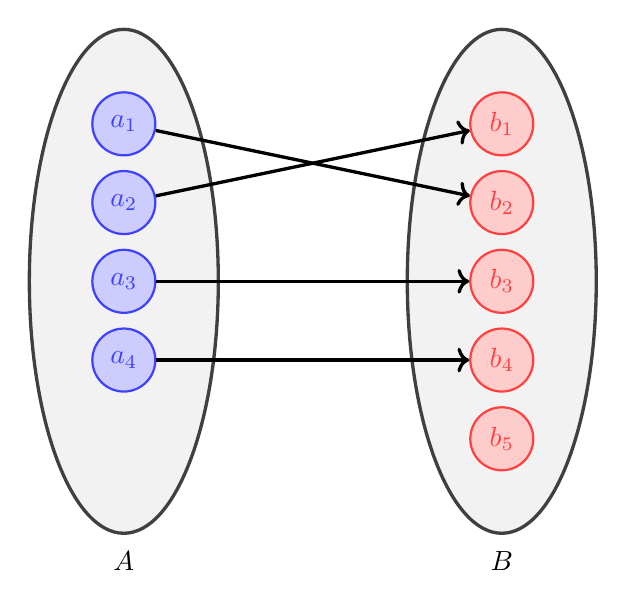
\begin{tikzpicture}[scale=0.8]
		\tikzstyle{blue-node}=[color=blue!75,fill=blue!20,thick,circle, draw, minimum width=0.8cm]
		\tikzstyle{red-node}=[color=red!75,fill=red!20,thick,circle, draw, minimum width=0.8cm]
		\tikzstyle{parent}=[color=black!75,fill=black!5,very thick]
		\tikzstyle{mapsto}=[->,very thick]
		% set A
		\draw [parent] (-2,0) ellipse (1.5cm and 4cm);
		\node [blue-node] at (-2,2.5) (a1) {$a_1$};
		\node [blue-node] at (-2,1.25) (a2) {$a_2$};
		\node [blue-node] at (-2,0) (a3) {$a_3$};
		\node [blue-node] at (-2,-1.25) (a4) {$a_4$} (-2,-4.75) node[anchor=south,color=black] {$A$};
		% set B
		\draw [parent] (4,0) ellipse (1.5cm and 4cm);
		\node [red-node] at (4,2.5) (b1) {$b_1$};
		\node [red-node] at (4,1.25) (b2) {$b_2$};
		\node [red-node] at (4,0)(b3) {$b_3$};
		\node [red-node] at (4,-1.25) (b4) {$b_4$};
		\node [red-node] at (4,-2.5) (b5) {$b_5$} (4,-4.75) node[anchor=south,color=black] {$B$};
		% mapsto
		\draw [mapsto] (a1) -- (b2);
		\draw [mapsto] (a2) -- (b1);
		\draw [mapsto] (a3) -- (b3);
		\draw [mapsto] (a4) -- (b4);
	\end{tikzpicture}
	\caption{Example of an injective function}
	\label{sketch-injective-function}
\end{figure}

\begin{exm}\label{exm-surjective-function}
	Let $f:\mathbb{R}\rightarrow\mathbb{R},f(x)=2x+3$. Is this function surjective?
	\begin{flushleft}
		\textbf{Answer}: For any $y=f(x)\in\mathbb{R}$ there exists an $x=\frac{y-3}{2}$
		such that
		\begin{align*}
			f(x) & = 2\left(\frac{y-3}{2}\right)+3 \\
			     & = y - 3 + 3                     \\
			     & = y
		\end{align*}
		This proves that the function $f(x)=2x+3$ is surjective since $\text{Im}(f)=\mathbb{R}$.
		With respect to \pref{figure}{sketch-surjective-function} this means that
		every value from the codomain is taken on \textit{at least} once.
	\end{flushleft}
	\begin{rem}
		The strategy for determining whether a function is
		surjective or not boils down to solving the original function definition
		for $x$ and plugging in this expression in $f(x)$. If you can show that
		$f(x)=y$ then you are done, if not then the function is not surjective.
	\end{rem}
\end{exm}

\begin{figure}[ht!]
	\centering
	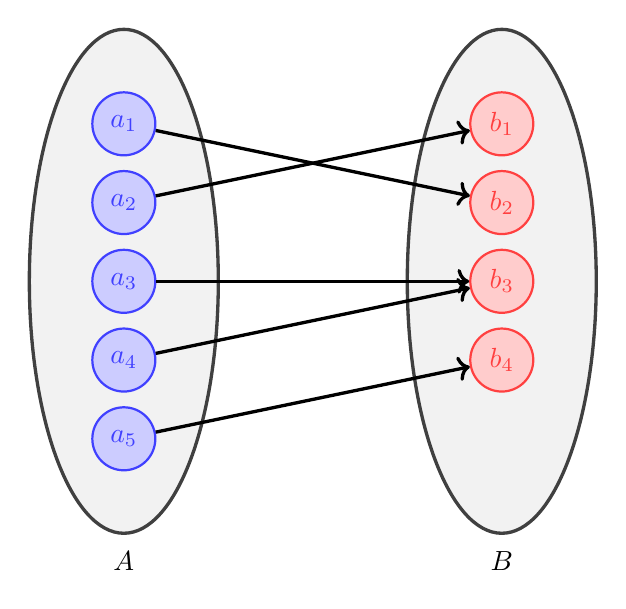
\begin{tikzpicture}[scale=0.8]
		\tikzstyle{blue-node}=[color=blue!75,fill=blue!20,thick,circle, draw, minimum width=0.8cm]
		\tikzstyle{red-node}=[color=red!75,fill=red!20,thick,circle, draw, minimum width=0.8cm]
		\tikzstyle{parent}=[color=black!75,fill=black!5,very thick]
		\tikzstyle{mapsto}=[->,very thick]
		% set A
		\draw [parent] (-2,0) ellipse (1.5cm and 4cm);
		\node [blue-node] at (-2,2.5) (a1) {$a_1$};
		\node [blue-node] at (-2,1.25) (a2) {$a_2$};
		\node [blue-node] at (-2,0) (a3) {$a_3$};
		\node [blue-node] at (-2,-1.25) (a4) {$a_4$};
		\node [blue-node] at (-2,-2.5) (a5) {$a_5$} (-2,-4.75) node[anchor=south,color=black] {$A$};
		% set B
		\draw [parent] (4,0) ellipse (1.5cm and 4cm);
		\node [red-node] at (4,2.5) (b1) {$b_1$};
		\node [red-node] at (4,1.25) (b2) {$b_2$};
		\node [red-node] at (4,0)(b3) {$b_3$};
		\node [red-node] at (4,-1.25) (b4) {$b_4$} (4,-4.75) node[anchor=south,color=black] {$B$};
		% mapsto
		\draw [mapsto] (a1) -- (b2);
		\draw [mapsto] (a2) -- (b1);
		\draw [mapsto] (a3) -- (b3);
		\draw [mapsto] (a4) -- (b3);
		\draw [mapsto] (a5) -- (b4);
	\end{tikzpicture}
	\caption{Example of an surjective function}
	\label{sketch-surjective-function}
\end{figure}

\begin{exm}\label{exm-bijective-function}
	Let $f:\mathbb{R}\rightarrow\mathbb{R},f(x)=2x+3$. Is this function bijective?
	\begin{flushleft}
		\textbf{Answer}: From \pref{example}{exm-injective-function} and
		\pref{example}{exm-surjective-function} we can deduce that since the function
		is injective and surjective, that it is bijective as well. With respect
		to \pref{figure}{sketch-bijective-function} this means that every value
		from the codomain is taken on \textit{exactly} once.
	\end{flushleft}
\end{exm}

\begin{figure}[ht!]
	\centering
	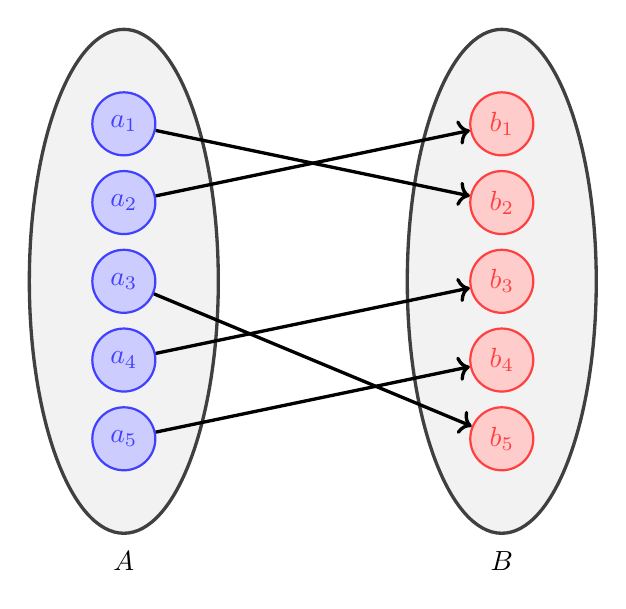
\begin{tikzpicture}[scale=0.8]
		\tikzstyle{blue-node}=[color=blue!75,fill=blue!20,thick,circle, draw, minimum width=0.8cm]
		\tikzstyle{red-node}=[color=red!75,fill=red!20,thick,circle, draw, minimum width=0.8cm]
		\tikzstyle{parent}=[color=black!75,fill=black!5,very thick]
		\tikzstyle{mapsto}=[->,very thick]
		% set A
		\draw [parent] (-2,0) ellipse (1.5cm and 4cm);
		\node [blue-node] at (-2,2.5) (a1) {$a_1$};
		\node [blue-node] at (-2,1.25) (a2) {$a_2$};
		\node [blue-node] at (-2,0) (a3) {$a_3$};
		\node [blue-node] at (-2,-1.25) (a4) {$a_4$};
		\node [blue-node] at (-2,-2.5) (a5) {$a_5$} (-2,-4.75) node[anchor=south,color=black] {$A$};
		% set B
		\draw [parent] (4,0) ellipse (1.5cm and 4cm);
		\node [red-node] at (4,2.5) (b1) {$b_1$};
		\node [red-node] at (4,1.25) (b2) {$b_2$};
		\node [red-node] at (4,0)(b3) {$b_3$};
		\node [red-node] at (4,-1.25) (b4) {$b_4$};
		\node [red-node] at (4,-2.5) (b5) {$b_5$} (4,-4.75) node[anchor=south,color=black] {$B$};
		% mapsto
		\draw [mapsto] (a1) -- (b2);
		\draw [mapsto] (a2) -- (b1);
		\draw [mapsto] (a3) -- (b5);
		\draw [mapsto] (a4) -- (b3);
		\draw [mapsto] (a5) -- (b4);
	\end{tikzpicture}
	\caption{Example of an bijective function}
	\label{sketch-bijective-function}
\end{figure}

\begin{exm}\label{exm-injective-surjective-bijective}
	Determine whether the following functions are injective, surjective or
	bijective\footnote{You may also consult \pref{figure}{sktech:exm-1:4} for
		additional help.}:
	\begin{enumerate}
		\item[1.)] $f(x):\mathbb{R}^+\rightarrow\mathbb{R}^+,x\mapsto x^2-1$
		\item[2.)] $g(x):\mathbb{R}^+\rightarrow\mathbb{R},x\mapsto x^2-1$
		\item[3.)] $h(x):\mathbb{R}\rightarrow\mathbb{R}^+,x\mapsto x^2-1$
		\item[4.)] $i(x):\mathbb{R}\rightarrow\mathbb{R},x\mapsto x^2-1$
	\end{enumerate}
	\begin{flushleft}
		\textbf{Answer:} TODO
	\end{flushleft}
\end{exm}

\begin{definition}\label{def-inverse-function}
	Let $f:\mathcal{D}\to\mathcal{C}$. We say that $f$ is invertible if there exists
	$f^{-1}:\mathcal{C}\to\mathcal{D}$ such that
	\begin{equation}
		\forall x\in\mathcal{D}:(f^{-1}\circ f)(x)=x
		\land \forall y\in\mathcal{C}:(f \circ f^{-1})(y)=y
	\end{equation}
	If that's the case, we call $f^{-1}$ the inverse function of $f$.
\end{definition}

\begin{thm}\label{thm-inverse-function}
	A function $f$ is invertible, \textit{iff} it is bijective.
\end{thm}

\begin{rem}\label{rem-sqrt-function}
	In school we learnt that the function
	\begin{equation}\label{eq-sqrt-function}
		f:\mathbb{R}^+\to\mathbb{R}^+,x\mapsto\sqrt{x}
	\end{equation}
	is the inverse function of
	\begin{equation}\label{eq-pow-function}
		f:\mathbb{R}\to\mathbb{R}^+,x\mapsto x^2
	\end{equation}
	Notice that the square root function in \pref{equation}{eq-sqrt-function} is
	only defined for positive values on $\mathbb{R}$. This is because the principal
	square root is positive:
	\begin{equation}\label{eq-sqrt-abs-function}
		\sqrt{x^2}=\abs{x}
	\end{equation}
	You may have been taught in physics that the square root function can take on
	two values, \textit{i.e.} $\sqrt{x^2}=\pm x$, for example
	\begin{equation*}
		f(x=9)=\sqrt{9}\implies x=3 \lor x=-3
	\end{equation*}
	But \pref{theorem}{thm-inverse-function} states that inverse functions are
	bijective\footnote{To satisfy this old notion, the square root function would
		have to be strictly surjective, see also \pref{figure}{sketch-surjective-function}.}.
	\begin{figure}[h!]
		\centering
		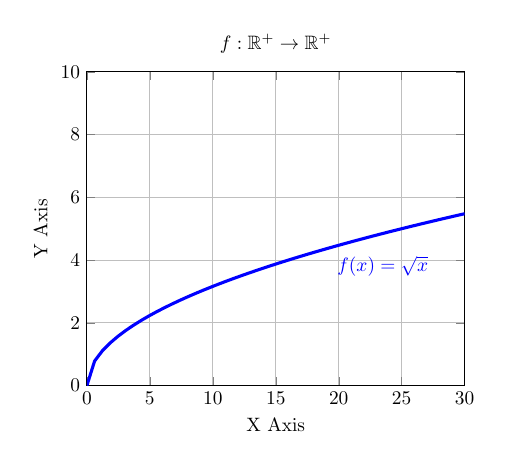
\begin{tikzpicture}[scale=0.7]
			\begin{axis}[
					xmax=30,
					xmin=0,
					ymax=10,
					ymin=0,
					samples=50,
					grid=major,
					xlabel={X Axis},
					ylabel={Y Axis},
					title={$f:\mathbb{R}^+\to\mathbb{R}^+$}
				]
				\addplot[blue, ultra thick,domain=0:30]{sqrt(x)} node[anchor=north west,pos=0.65] {$f(x)=\sqrt{x}$};
			\end{axis}
		\end{tikzpicture}
		\caption{The square root function only operates with positive numbers}
		\label{sketch:rem-sqrt-function}
	\end{figure}
	So, while it is sometimes convenient to follow the convention in \pref{equation}{eq-sqrt-abs-function},
	strictly speaking the square root function only ever takes on positive values
	(\textit{cf.} \pref{figure}{sketch:rem-sqrt-function}).
\end{rem}

\begin{definition}\label{def-floor-function}
	The floor function is defined by
	\begin{equation}
		\ffloor(x)=\floor{x}\defines\max\left\{m\in\mathbb{Z}\setbuild m\leq x\right\}
	\end{equation}
\end{definition}

\begin{definition}\label{def-ceiling-function}
	The ceiling function is defined by
	\begin{equation}
		\fceil(x)=\ceil{x}\defines\min\left\{n\in\mathbb{Z}\setbuild n\geq x\right\}
	\end{equation}
\end{definition}

\begin{definition}\label{def-dirichlet-function}
	The Dirichlet function is defined by
	\begin{equation}
		D(x)=\begin{cases}
			1\text{ if }x\in\mathbb{Q} \\
			0\text{ else }
		\end{cases}
	\end{equation}
\end{definition}

\begin{definition}\label{def-absolute-value-function}
	The absolute value function is defined by
	\begin{equation}
		\forall x\in\mathbb{R}: \abs{x}\defines\max\{x,-x\}=\begin{cases}
			x\text{ if } x \geq 0 \\
			-x \text{ else }
		\end{cases}
	\end{equation}
\end{definition}

\begin{thm}\label{thm-absolute-value-properties}
	Below are listed some of the properties related to the absolute value; for
	any $x\in\mathbb{R}$ the following holds:
	\begin{enumerate}
		\item $\abs{x} \geq 0$
		\item $\abs{x} \geq \pm x$
		\item $\abs{x} = \abs{-x}$
		\item $\abs{x} = 0 \iff x = 0$
		\item $\abs{xy} = \abs{x}\abs{y}$
		\item $\abs{x} + \abs{y} \geq \abs{x+y}$
		\item $\abs{x-y} \geq \abs[\big]{\abs{x}-\abs{y}}$
		\item $\abs{x} < M \iff -M < x < M$
	\end{enumerate}
\end{thm}

\begin{proof}
	Of theorem (\ref{thm-absolute-value-properties}).
	\begin{flushleft}
		In this proof we will only show property 6 of this theorem which is also
		known as the triangle inequality. From property 2 it follows that the sum
		of $\abs{x}\geq x$ and $\abs{y}\geq y$ equals
		\begin{equation}\label{tmp-absolute-value-properties:1}
			\abs{x} + \abs{y} \geq x + y
		\end{equation}
		Likewise, from $\abs{x}\geq -x$ and $\abs{y}\geq -y$ it follows that
		\begin{equation}\label{tmp-absolute-value-properties:2}
			\abs{x} + \abs{y} \geq -(x+y)
		\end{equation}
		Thus, by definition (\ref{def-absolute-value-function}) and equation
		(\ref{tmp-absolute-value-properties:1}) and (\ref{tmp-absolute-value-properties:2})
		we can conclude that
		\begin{equation*}
			\abs{x} + \abs{y} \geq \abs{x+y}
		\end{equation*}
	\end{flushleft}
\end{proof}

\begin{rem}
	A geometric interpretation of the absolute value function $\abs{x}$ is the
	distance from $x$ to $0$. Similarly, the absolute value of the difference
	$\abs{x-y}$ can be interpreted as the distance between $x$ and $y$. See also
	\hyperref[subsec-metric-spaces]{the subsection for metric spaces} for more
	more information on distances.
\end{rem}


\subsection{Limit Prerequisites}\label{subsec-limit-prerequisites}

\begin{definition}\label{def-interval-notation}
    As opposed to closed intervals, open and half-open intervals contain infinitely
    many elements. The $\infty$ symbol always needs to be paired with a parenthesis
    rather than a bracket because it is technically incorrect to think of infinity
    as a number. So far, we haven't agreed on a formal definition for the concept
    of infinity, but it will become important later when we discuss limits in more
    detail.
    \begin{enumerate}
        \item $(a,b)\defines\left\{x\setbuild a < x < b\right\}       \quad \text{(Open interval)}$
        \item $(a,b]\defines\left\{x\setbuild a < x \leq b\right\}    \quad \text{(Half-open interval)}$
        \item $[a,b)\defines\left\{x\setbuild a \leq x < b\right\}    \quad \text{(Half-closed interval)}$
        \item $[a,b]\defines\left\{x\setbuild a \leq x \leq b\right\} \quad \text{(Closed interval)}$
    \end{enumerate}
\end{definition}

\begin{definition}\label{def-epsilon-neighborhood}
    Let $a\in\mathbb{R}$ and $\varepsilon > 0$. Then the open interval 
    $(a-\varepsilon,a+\varepsilon)$ is called the epsilon neighborhood of $a$
    and is denoted by
    \begin{equation}
        \mathcal{U}_\varepsilon(a)\defines
        \left\{x \setbuild x\in\mathbb{R},\abs{x-a}<\varepsilon \right\}=
        (a-\varepsilon,a+\varepsilon)
    \end{equation}
\end{definition}

\begin{rem}\label{rem-epsilon-neighborhood}
    In reference to property 8 of theorem (\ref{thm-absolute-value-properties})
    we can note that
    \begin{equation}
        x\in(a-\varepsilon,a+\varepsilon) \iff \abs{x-a} < \varepsilon
    \end{equation}
\end{rem}

\begin{definition}\label{def-epsilon-punctured-neighborhood}
    Let $a\in\mathbb{R}$. For $\varepsilon>0$ we define the punctured epsilon 
    neighborhood of $a$, denoted by 
    \begin{equation}
        \mathcal{U}_{\varepsilon}^{\bolddot}(a)\defines
        \left\{x \setbuild x\in\mathbb{R}, 0<\abs{x-a}<\varepsilon\right\}=
        (a-\varepsilon,a+\varepsilon)\setminus\{a\}
    \end{equation}
\end{definition}

\begin{definition}\label{def-limit-point}
    Let $M\subset\mathbb{R}$ and $a\in\mathbb{R}$. Then, $a$ is called a limit 
    point\footnote{Or cluster point} of $M$ \textit{iff}
    \begin{equation}
        \bigwedge_{\varepsilon>0}(M\cap\mathcal{U}_\varepsilon^{\bolddot}\neq\emptyset)
    \end{equation}
\end{definition}

\begin{definition}\label{def-isolated-point}
    In contrast to definition (\ref{def-limit-point}), we call $a$ an isolated point
    of $M$ \textit{iff}
    \begin{equation}
        \neg\bigwedge_{\varepsilon>0}(M\cap\mathcal{U}_\varepsilon^{\bolddot}\neq\emptyset)
        \iff
        \bigvee_{\varepsilon>0}(M\cap\mathcal{U}_\varepsilon^{\bolddot}=\emptyset)
    \end{equation}
    \textit{i.e.} $a\in M\subset\mathbb{R}$ and $a$ is not a limit point.
\end{definition}

\begin{rem}
    If $a$ is an isolated point of $M$, then \cite[p.67]{wuest2009}
    \begin{align*}
        a\in M:\mathcal{U}_\varepsilon(a)
        &=(\{a\}\cup\mathcal{U}_\varepsilon^{\bolddot})\cap M \\
        &=(\{a\}\cap M)\cup(\mathcal{U}_\varepsilon^{\bolddot}\cap M) \\
        &=\{a\}
    \end{align*}
    Therefore, in the neighborhood of $a$ are no other elements of the set $M$.
\end{rem}

\begin{exm}\label{exm-limit-points}
    Find the set of all limit points for
    \begin{enumerate}
        \item $A\defines\displaystyle\bigcup_{n\in\mathbb{N}}\left(\frac{1}{n},2-\frac{1}{n}\right)$
        \item $B\defines\left\{x\in\mathbb{R}\setbuild x=n+\frac{1}{m}\quad\text{($n,m$ appropriate)}\right\}$
    \end{enumerate}
    \begin{flushleft}
        \textbf{\nth{1} Answer:} TODO
    \end{flushleft}
    \begin{flushleft}
        \textbf{\nth{2} Answer:} TODO
    \end{flushleft}
\end{exm}

\begin{definition}\label{def-bounded-sets}
    Let $A \subseteq\mathbb{R}$ be a set.
    \begin{enumerate}
        \item Then $A$ is called bounded from above if there exists $M\in\mathbb{R}$ 
        such that $x\leq M$ for any $x\in A$.
        \item Similarly, $A$ is bounded from below if there exists $m\in\mathbb{R}$ 
        such that $x\geq M$ for any $x\in A$.
        \item Finally, $A$ is called bounded if it is bounded from above and below.
        \footnote{Notice that the boundary points in this definition
        lay no claim to uniqueness.}
    \end{enumerate}
\end{definition}

\begin{exm}\label{exm-bounded-sets:1}
    \hfill
    \begin{enumerate}
        \item Consider the set of natural numbers: $\mathbb{N}$ is not bounded from above, but 
        below, \textit{i.e.} $1$ is a lower bound of $\mathbb{N}$.
        \item Let $A=(-3,2]$. Then this set is bounded from above and below.
        \item Let $B=\left\{\frac{1}{n}\setbuild n\in\mathbb{N}\right\}$. Then this
        set is bounded from above by $1$, and bounded from below by $0$.
    \end{enumerate}
\end{exm}

\begin{definition}\label{def-supremum-infimum-sets}
    Let $A\subset\mathbb{R}$ be a set.
    \begin{enumerate}
        \item $S$ is called the supremum of $A$ if it is the smallest upper bound 
        of $A$, and is denoted by $S=\sup(A)$.
        \item $I$ is called the infimum of $A$ if it is the largest lower bound 
        of $A$, and is denoted by $I=\inf(A)$.
    \end{enumerate}
\end{definition}

\begin{exm}\label{exm-bounded-sets:2}
    Consider the sets from \pref{example}{exm-bounded-sets:1}. Then\footnote{Remark:
    $\mathbb{N}\defines\{1,2,3,\dots\}$}
    \begin{enumerate}
        \item $\inf(\mathbb{N})=1$
        \item $\inf(A)=-3$ and $\sup(A)=2$
        \item $\inf(B)=0$ and $\sup(B)=1$
    \end{enumerate}
\end{exm}

\begin{definition}\label{def-maximum-minimum}
    Let $A\subset\mathbb{R}$ be a set.
    \begin{enumerate}
        \item If $S=\sup(A)$, then $S\in A$ is also a maximum of $A$ and is denoted by $S=\max(A)$.
        \item If $I=\inf(A)$, then $I\in A$ is also a minimum of $A$ and is denoted by $I=\min(A)$.
    \end{enumerate}
\end{definition}

\begin{exm}\label{exm-bounded-sets:3}
    Expanding on the results from example (\ref{exm-bounded-sets:2}), we note that
    \begin{enumerate}
        \item $\min(\mathbb{N})=1$
        \item $\min(A)=\text{\gls{dne}}$ and $\max(A)=2$
        \item $\min(B)=\text{\gls{dne}}$ and $\max(B)=1$
    \end{enumerate}
\end{exm}


\subsection{Limits}\label{subsec-limits}

\begin{definition}\label{def-epsilon-delta-definition-limit}
    Let $f(x)$ be a function with $a,b\in\mathbb{R}$ with $a$ as a limit point of $\domain{f}$.
    Then the the function $f$ has the limit $b$ as $x$ approaches $a$, \textit{i.e.}    
    \begin{equation}
        \bigwedge_{\varepsilon>0}\bigvee_{\delta>0}\bigwedge_{x\in\domain{f}} 
        \left(0<\abs{x-a}<\delta\implies\abs{f(x)-b}<\varepsilon\right)
    \end{equation}
    The limit of this function is denoted by
    \begin{equation}
        \lim_{x\to a}f(x)=b,
    \end{equation}
\end{definition}

\begin{rem}
    The equation $\displaystyle\lim_{x\to a}f(x)=b$ is equivalent to the following
    expressions:
    \begin{enumerate}
        \item For $f$ there exists a limit (point) at $a$.
        \item This limit of $f$ is equal to $b$.
    \end{enumerate}
    In other words, $f$ has a limit at $a$ if
    \begin{equation*}
        \bigvee_{b\in\mathbb{R}}\bigwedge_{\varepsilon>0}\bigvee_{\delta>0}\bigwedge_{x\in\domain{f}} 
        \left(0<\abs{x-a}<\delta \implies \abs{f(x)-b}<\varepsilon\right)
    \end{equation*}
\end{rem}

\begin{exm}\label{exm-epsilon-delta-definition-limit:1}
    Show that 
    \begin{equation*}
        \lim_{x\to3}\frac{x-1}{2}=1
    \end{equation*}
    by using the epsilon-delta definition for limits.
    \begin{flushleft}
        \textbf{Answer}: Let $\varepsilon>0$ and $b\in\mathbb{R}$. Take 
        $\delta\defines2\varepsilon$; Then $\abs{x-3}<\delta$, which implies
        \begin{align*}
            \abs{f(x)-b}&=\abs[\Bigg]{\frac{x-1}{2}-1}\\
                        &=\frac{\abs{x-3}}{2}\\
                        &<\frac{\delta}{2}\\
                        &=\varepsilon
        \end{align*}
    \end{flushleft}
\end{exm}

\begin{exm}\label{exm-epsilon-delta-definition-limit:2}
    Show that for some $a\in\mathbb{R}$,
    \begin{equation*}
        \lim_{x\to a}\sin(x)=\sin(a)
    \end{equation*}
    by using the epsilon-delta definition for limits.
    \begin{flushleft}
        \textbf{Answer}: Let $\varepsilon>0$ and $b\in\mathbb{R}$. Take 
        $\varepsilon\defines\delta$ such that $\abs{x-a}<\delta$. Further, recall that
        \begin{align*}
            &\text{(A)}:\forall\alpha\in\mathbb{R}:\abs{\cos(\alpha)}\leq1\\
            &\text{(B)}:\forall\alpha\in\mathbb{R}:\abs{\sin(\alpha)}\leq\abs{\alpha}
        \end{align*}
        \begin{align*}
            \abs{f(x)-b}&=\abs{\sin(x)-\sin(a)}\\
                        &=\abs[\Bigg]{2\sin\left(\frac{x-a}{2}\right)\cos\left(\frac{x+a}{2}\right)}\\
                        &=2\cdot\abs[\Bigg]{\sin\left(\frac{x-a}{2}\right)}\abs[\Bigg]{\cos\left(\frac{x+a}{2}\right)}\\
                        &\leq 2\cdot\frac{\abs{x-a}}{2} && \text{note (A) \& (B)}\\
                        &=\varepsilon
        \end{align*}
    \end{flushleft}
\end{exm}

\begin{exm}\label{exm-epsilon-delta-definition-limit:3}
    Show \cite[p.69]{wuest2009} that the function $f(x)=\tfrac{x^2-3x+2}{x(x-1)}$
    with $x\in\mathbb{R}\setminus\{0,1\}$ has the limit $b=-1$ as $x\to1$.
    \begin{flushleft}
        \textbf{Answer}: Let $\varepsilon>0$.
        \begin{align}
            \abs{f(x)-(-1)}&=\abs[\Bigg]{\frac{x^2-3x+2}{x(x-1)}+1}\nonumber\\
                           &=\abs[\Bigg]{\frac{(x-2)(x-1)}{x(x-1)}+1}\nonumber\\
                           &=\abs[\Bigg]{\frac{x-2}{x}+1}\nonumber\\
                           &=\abs[\Bigg]{\frac{2x-2}{x}}\nonumber\\
                           &=\frac{2}{\abs{x}}\cdot\abs{x-1}\label{eq3-epsilon-delta-definition-limit:1}
        \end{align}
        Since we aim for the neighborhood of $x=1$ we can impose the following
        restriction on this inequality:
        \begin{equation}\label{eq3-epsilon-delta-definition-limit:2}
            0<\abs{x-1}<\frac{1}{2}
        \end{equation}
        This in turn implies
        \begin{align}
            \abs{x}&=\abs{x-1+1}\nonumber\\
                   &\geq1-\abs{x-1}\nonumber\\
                   &>1-\frac{1}{2} && \text{\pref{equation}{eq3-epsilon-delta-definition-limit:2}}\nonumber\\
                   &=\frac{1}{2}\label{eq3-epsilon-delta-definition-limit:3}
        \end{align}
        Hence,
        \begin{align}
            \abs{f(x)-b}&=\frac{2}{\abs{x}}\cdot\abs{x-1} && \text{\pref{equation}{eq3-epsilon-delta-definition-limit:1}}\nonumber\\
                        &<\frac{2}{\tfrac{1}{2}}\cdot\abs{x-1} && \text{\pref{equation}{eq3-epsilon-delta-definition-limit:3}}\nonumber\\
                        &=4\cdot\abs{x-1}\label{eq3-epsilon-delta-definition-limit:4}
        \end{align}
    \end{flushleft}
    Let $q(\varepsilon)\defines\min\left\{\tfrac{\varepsilon}{4},\tfrac{1}{2}\right\}$.
    Then for all $\varepsilon>0$ there exists a $\delta\defines q(\varepsilon)$ such that
    for $x\in\domain{f}$ it follows that
    \begin{align*}
        0<\abs{x-1}<\delta \implies \abs{f(x)-(-1)}&<4\cdot\abs{x-1}&&\text{\pref{equation}{eq3-epsilon-delta-definition-limit:4}}\\
                                                   &<4\cdot\frac{\varepsilon}{4}\\
                                                   &=\varepsilon
    \end{align*}
\end{exm}

\begin{exm}\label{exm-epsilon-delta-definition-limit:4}
    Show that the function $f(x)=\tfrac{x^2-4x+3}{2x-6}$ with $x\in\mathbb{R}\setminus\{3\}$
    has the limit $b=1$ as $x\to3$.
    \begin{flushleft}
        \textbf{Answer}: Let $\varepsilon>0$. Define $\delta\defines2\varepsilon$,
        such that $\abs{x-3}<\delta$, wherefore
        \begin{align*}
            \abs{f(x)-b}&=\abs[\Bigg]{\frac{x^2-4x+3}{2x-6}-1}\\
                        &=\abs[\Bigg]{\frac{(x-1)(x-3)}{2(x-3)}-1}\\
                        &=\abs[\Bigg]{\frac{1}{2}(x-1)-1}\\
                        &=\abs[\Bigg]{\frac{1}{2}x-\frac{3}{2}}\\
                        &=\frac{1}{2}\abs{x-3}\\
                        &<\frac{1}{2}\cdot2\varepsilon\\
                        &=\varepsilon
        \end{align*}
    \end{flushleft}
\end{exm}

\begin{exm}\label{exm-epsilon-delta-definition-limit:5}
    Show that for $a>0$ ($a\in\mathbb{R}$),
    \begin{equation*}
        \sqrt{x}\tolim{x}{a}\sqrt{a}
    \end{equation*}
    \begin{flushleft}
        \textbf{Answer}: Let $\varepsilon>0$. When we define $\delta\defines\min\left\{a,\varepsilon\sqrt{a}\right\}$,
        then $\abs{x-a}<\delta$ implies that
        \begin{align*}
            \abs{f(x)-b}&=\abs[\big]{\sqrt{x}-\sqrt{a}}\\
                        &=\frac{\abs[\big]{\sqrt{x}-\sqrt{a}}\left(\sqrt{x}+\sqrt{a}\right)}{\sqrt{x}+\sqrt{a}}\\
                        &=\frac{\abs{x-a}}{\sqrt{x}+\sqrt{a}}\\
                        &<\frac{\abs{x-a}}{\sqrt{a}}\\
                        &<\frac{\varepsilon\sqrt{a}}{\sqrt{a}}\\
                        &=\varepsilon
        \end{align*}
        Therefore,
        \begin{equation*}
            \lim_{x\to a}\sqrt{x}=\sqrt{a}
        \end{equation*}
    \end{flushleft}
\end{exm}

\begin{rem}\label{rem-undefined-limits}
    Examples of functions where \pref{definition}{def-epsilon-delta-definition-limit} breaks:
    \begin{enumerate}
        \item For any $a\in\mathbb{Z}$, the limit of $f(x)=\floor{x}$ does not exists.
        \item The limit $\displaystyle\lim_{x\to0}\tfrac{1}{x}$ does not exists.
        \item The limit $\displaystyle\lim_{x\to0}\tfrac{1}{x^2}$ does not exists.
        \item The limit $\displaystyle\lim_{x\to0}\sin\left(\tfrac{1}{x}\right)$ does not exists.
    \end{enumerate}
\end{rem}

\begin{thm}\label{thm-limit-arithmetic}
    Let $\displaystyle\lim_{x \to a}f(x) = b_1$ and $\displaystyle\lim_{x \to a}g(x) = b_2$
    be two well-defined limits. Then the following statements hold:
    \begin{enumerate}
        \item $c \cdot f(x) \tolim{x}{a} c \cdot b_1 \quad (c\in\mathbb{R})$
        \item $f(x) + g(x) \tolim{x}{a} b_1 + b_2$
        \item $f(x) \cdot g(c) \tolim{x}{a} b_1 \cdot b_2$
        \item $\tfrac{f(x)}{g(x)} \tolim{x}{a} \tfrac{b_1}{b_2} \quad (b_2 \neq 0)$
    \end{enumerate}
\end{thm}


\begin{proof}
    Of \pref{theorem}{thm-limit-arithmetic}.
    \begin{flushleft}
        \textbf{\nth{2} Property}. From \pref{definition}{def-epsilon-delta-definition-limit}
        we can note that
        \begin{align*}
            &\forall\varepsilon>0\;\exists\delta_1>0:\,\abs{x-a}<\delta_1\implies\abs{f(x)-b_1}<\frac{\varepsilon}{2}\\
            &\forall\varepsilon>0\;\exists\delta_2>0:\,\abs{x-a}<\delta_2\implies\abs{g(x)-b_2}<\frac{\varepsilon}{2}
        \end{align*}        
        Define $\delta\defines\min\{\delta_1,\delta_2\}$ Then, if $\abs{x-a}<\delta$,
        it follows from the triangle inequality that
        \begin{align*}
            \abs{f(x)+g(x)-(b_1+b_2)}&=\abs{(f(x)-b_1)+(g(x)-b_2)}\\
                                     &\leq\abs{f(x)-b_1}+\abs{g(x)-b_2}\\
                                     &<\frac{\varepsilon}{2}+\frac{\varepsilon}{2}\\
                                     &=\varepsilon
        \end{align*}
    \end{flushleft}
\end{proof}

\begin{exm}
    Find the limit of
    \begin{equation*}
        \lim_{x \to 0}\left(\arctan\left(2\sqrt{\frac{\cos(x)}{3x+4}}\right)\right)=\frac{\pi}{4}
    \end{equation*}
    \begin{flushleft}
        \textbf{Answer}: TODO
    \end{flushleft}
\end{exm}

\begin{thm}\label{thm-absolute-value-of-limit:1}
    If $f(x) \tolim{x}{a} 0$, then this is equivalent to
    $\abs{f(x)} \tolim{x}{a} 0$.
\end{thm}

\begin{thm}\label{thm-absolute-value-of-limit:2}
    Let $b\in\mathbb{R}$. If $f(x) \tolim{x}{a} b$, then 
    this implies $\abs{f(x)} \tolim{x}{a} \abs{b}$.
\end{thm}

\begin{rem}
    Note that the opposite direction of \pref{theorem}{thm-absolute-value-of-limit:2}
    is in general not true. A counter example for this would be the 
    \hyperref[def-dirichlet-function]{Dirichlet function}.
\end{rem}

\begin{proof}
    Of \pref{theorem}{thm-absolute-value-of-limit:2}.
    \begin{flushleft}
        Let $\varepsilon>0$. Then $\abs{x-a}<\delta$ implies that
        \begin{align*}
            \abs[\big]{\abs{f(x) - \abs{b}}} &\leq \abs{f(x) - b} \\
                                             &<\varepsilon
        \end{align*}
        by using the reverse triangle inequality for absolute values.
    \end{flushleft}
\end{proof}

\begin{thm}\label{thm-limit-monotonicity}
    Let $f(x) \geq g(x)$ for any $x\in\mathcal{U}_{\varepsilon}^{\bolddot}(a)$. 
    If the limit of $f(x)$ and $g(x)$ exist, then
    \begin{equation*}
        \lim_{x \to a}f(x) \geq \lim_{x \to a}g(x)
    \end{equation*}
\end{thm}

\begin{rem}
    As for \pref{theorem}{thm-limit-monotonicity}, if $f(x) \geq 0$,
    then
    \begin{equation*}
        \lim_{x \to a}f(x) \geq 0
    \end{equation*}
\end{rem}

\begin{rem}
    \pref{Theorem}{thm-limit-monotonicity} does not hold if we replace the greater
    than or equal to inequality with a strictly greater than inequality.
\end{rem}

\begin{thm}\label{thm-unique-limit}
    If the limit of $\displaystyle\lim_{x\to a}f(x)=b\in\mathbb{R}$ exists, then $b$ is unique.
\end{thm}

\begin{proof}
    Of \pref{theorem}{thm-unique-limit}.
    \begin{flushleft}
        Assume \gls{wlog} that $b<c$ are both limits of this function. Define
        $\varepsilon\defines\tfrac{c-b}{3}>0$. Then by 
        \pref{definition}{def-epsilon-delta-definition-limit} we have that
        \begin{equation}\label{eq-unique-limit:1}
            \exists\delta_1\text{ s.t. }a-\delta_1<x<a+\delta_1 \implies b-\varepsilon<f(x)<b+\varepsilon
        \end{equation}
        Likewise we know that
        \begin{equation}\label{eq-unique-limit:2}
            \exists\delta_2\text{ s.t. }a-\delta_1<x<a+\delta_1 \implies c-\varepsilon<f(x)<c+\varepsilon
        \end{equation}
    \end{flushleft}
    Therefore by \pref{equation}{eq-unique-limit:1} and \pref{equation}{eq-unique-limit:2},
    it follows that
    \begin{equation*}
        \left(f(x)<b+\varepsilon<c+\varepsilon\right)\land\left(c+\varepsilon<f(x)\right)
    \end{equation*}
    which is a contradiction. 
\end{proof}

\begin{thm}\label{def-limit-is-bounded}
    If the limit of $\displaystyle\lim_{x\to a}f(x)=b\in\mathbb{R}$ exists, then
    $f$ is bounded in a neighborhood of $a$.
\end{thm}

\begin{thm}\label{thm-sandwich-theorem}
    Suppose that for any $x$ in a neighborhood of $a$
    \begin{equation*}
        h(x) \leq f(x) \leq g(x)
    \end{equation*}
    Further assume that
    \begin{equation*}
        \lim_{x \to a}h(x) = b = \lim_{x \to a}g(x)
    \end{equation*} 
    Then it follows that
    \begin{equation*}
        \lim_{x \to a}f(x) = b
    \end{equation*}
\end{thm}

\begin{proof}
    Of \pref{theorem}{thm-sandwich-theorem}.
    \begin{flushleft}
        Let $\varepsilon>0$. Take $\delta\defines\min\{\delta_1,\delta_2\}$ where
        \begin{align*}
            &0 < \abs{x - a} < \delta_1 \implies \abs{g(x) - b} < \varepsilon \iff b - \varepsilon < g(x) < b + \varepsilon, \\
            &0 < \abs{x - a} < \delta_2 \implies \abs{h(x) - b} < \varepsilon \iff b - \varepsilon < h(x) < b + \varepsilon
        \end{align*}
        Therefore, if $0 < \abs{x - a} < \delta$,
        \begin{equation*}
            b - \varepsilon < h(x) \leq f(x) \leq g(x) < b + \varepsilon
        \end{equation*}
        which is equivalent to
        \begin{equation*}
            \abs{f(x) - b} < \varepsilon \iff \lim_{x \to a}f(x) = b
        \end{equation*}
    \end{flushleft}
\end{proof}

\begin{thm}\label{thm-product-of-bounded-zero-limit}
    If $\displaystyle\lim_{x \to a}f(x) = 0$ and $g(x)$ is bounded in a neighborhood
    of $a$, then
    \begin{equation*}
        \lim_{x \to a} \left(f(x)\cdot g(x)\right) = 0
    \end{equation*}
\end{thm}

\begin{proof}
    Of \pref{theorem}{thm-product-of-bounded-zero-limit}.
    \begin{flushleft}
        Since $g(x)$ is bounded, we can write $\abs{g(x)} \leq M$. So,
        \begin{align*}
            &-M \leq \abs{g(x)} \leq M\\
            \implies
            &-M\cdot\abs{f(x)} \leq \abs{f(x)}\cdot\abs{g(x)} \leq M\cdot \abs{f(x)}\\
            \implies
            &-M\cdot \lim_{x \to a}\abs{f(x)} \leq  \lim_{x \to a}\left(\abs{f(x)}\cdot\abs{g(x)}\right) \leq M \cdot \lim_{x \to a}\abs{f(x)}\\
            \implies
            &-M \cdot 0 \leq \abs{f(x)}\cdot\abs{g(x)} \leq M \cdot 0 && \text{\pref{theorem}{thm-absolute-value-of-limit:1}} \\
            \implies
            & 0 \leq \abs{f(x)}\cdot\abs{g(x)} \leq 0 && \text{\pref{theorem}{thm-limit-arithmetic}}\\
            \implies
            &\lim_{x \to a}\left(\abs{f(x)}\cdot\abs{g(x)}\right)=0 && \text{\pref{theorem}{thm-sandwich-theorem}}\\
            \implies
            &\lim_{x \to a}\left(f(x)\cdot g(x)\right)=0 && \text{\pref{theorem}{thm-absolute-value-of-limit:1}} \\
        \end{align*}
    \end{flushleft}
\end{proof}

\begin{exm}
    The limit of the function 
    \begin{equation*}
        f(x) = x\cdot\sin\left(\frac{1}{x}\right)
    \end{equation*}
    as $x \to 0$ is
    \begin{equation*}
        \lim_{x \to 0}\left(x\cdot\sin\left(\frac{1}{x}\right)\right)=0
    \end{equation*}
    by \pref{theorem}{thm-product-of-bounded-zero-limit} since $\sin\left(\tfrac{1}{x}\right)$
    is bounded\footnote{But in and of itself not defined at $x=0$} by $[-1,1]$ 
    and the left factor of this function is $x=0$ as $x \to 0$.
\end{exm}

\begin{definition}\label{def-one-sided-limits}
    We denote the one-sided limit of the function $f(x)$ approached from the right by
    \begin{equation*}
        \lim_{x \to a^+}f(x)=b
    \end{equation*}
    if and only if
    \begin{equation}
        \forall\varepsilon>0\;\exists\delta>0:x\in(a,a+\delta)\implies\abs{f(x)-b}<\varepsilon
    \end{equation}
    Conversely, the left-sided limit is denoted by
    \begin{equation*}
        \lim_{x \to a^-}f(x)=b
    \end{equation*}
    if and only if
    \begin{equation}
        \forall\varepsilon>0\;\exists\delta>0:x\in(a-\delta,a)\implies\abs{f(x)-b}<\varepsilon
    \end{equation}
\end{definition}

\begin{rem}\label{rem-one-sided-limits}
    With respect to \pref{definition}{def-one-sided-limits}, note that there exist
    several equivalent notations. So, the right-sided limit of $f(x)$ can be denoted
    by
    \begin{equation*}
        \lim_{x \to a^+}f(x)=b
        \iff
        \lim_{x \underset{x>a}{\to} a}f(x)=b
        \iff
        \lim_{x\searrow  a}f(x)=b
    \end{equation*}
    Similarly, at times the left-sided limits may be denoted by
    \begin{equation*}
        \lim_{x \to a^-}f(x)=b
        \iff
        \lim_{x \underset{x<a}{\to} a}f(x)=b
        \iff
        \lim_{x \nearrow a}f(x)=b
    \end{equation*}
\end{rem}

\begin{thm}\label{thm-limit-exists-one-sided-limits}
    The limit of $f(x) \to b$ exists as $x \to a$ if and only if the left-sided
    limit as well as the right-sided limit of $f$ exists with
    \begin{equation}
        \lim_{x \to a}f(x)=b \iff \lim_{x \to a^+}f(x)=b=\lim_{x \to a^-}f(x)
    \end{equation}
\end{thm}

\begin{proof}
    Of \pref{theorem}{thm-limit-exists-one-sided-limits}.
    \begin{flushleft}
        TODO
    \end{flushleft}
\end{proof}

\begin{exm}\label{exm-important-sin-over-x-limit}
    Show that\footnote{This is a very useful limit that we are going to encounter
    more often in the near future.}
    \begin{equation}\label{eq-important-sin-over-x-limit}
        \lim_{x \to 0}\frac{\sin(x)}{x}=1
    \end{equation}
    \begin{flushleft}
        \textbf{Answer}: From figure (??) we can derive two observations:
        \begin{equation*}
            \forall x\in\left(0,\frac{\pi}{2}\right)\implies \sin(x)<x
        \end{equation*}
        Notice also that
        \begin{equation*}
            x < \tan(x)
        \end{equation*}
        So, this implies
        \begin{equation}\label{eq-important-sin-over-x-limit:1}
            \sin(x) < x < \tan(x)
        \end{equation}
        Furthermore, figure (??) reveals that
        \begin{equation*}
            \forall x\in\mathbb{R}:\abs{\sin(x)}\leq\abs{x}
        \end{equation*}
        From \pref{equation}{eq-important-sin-over-x-limit:1} follows that for all
        $\tfrac{\pi}{2}>x>0$:
        \begin{align*}
            \implies 
            &\frac{1}{\sin(x)} > \frac{1}{x} > \frac{1}{\tan(x)} \\
            \implies 
            &1 > \frac{\sin(x)}{x} > \cos(x) \\
            \implies 
            &1 > \lim_{x \to 0^+}\frac{\sin(x)}{x} > \lim_{x \to 0^+}\cos(x) \\
            \implies
            &1 > \lim_{x \to 0^+}\frac{\sin(x)}{x} > 1\\
            \implies 
            &\lim_{x \to 0^+}\frac{\sin(x)}{x}=1 && \text{theorem (\ref{thm-sandwich-theorem})}
        \end{align*}
        A similar argument can be made for 
        \begin{align*}
            \forall x\in\left(-\frac{\pi}{2},0\right):\lim_{x \to 0^-}\frac{\sin(x)}{x}=1
        \end{align*}
        Last but not least, \pref{theorem}{thm-limit-exists-one-sided-limits} ensures
        that the limit in \pref{equation}{eq-important-sin-over-x-limit} exists.
    \end{flushleft}
\end{exm}

\begin{thm}\label{thm-monotone-one-sided-limits}
    Assume that $f$ is monotone on some interval $[a,b]$. Then $f$ has one-sided
    limits at every point.
\end{thm}

\begin{definition}\label{def-infinity-limits}
    Let $f$ be a function such that\footnote{In other words, $\infty$ is a limit
    point of the domain of $f$}
    \begin{equation}
        \forall c\in\mathbb{R}: (c,\infty)\cap\domain{f}\neq\emptyset
    \end{equation}
    Next let $b\in\mathbb{R}$. We say that $f(x) \to b$ for $x \to \infty$ if and only if
    \footnote{Similarly, we can define the limit for $f(x) \to b$ as $x \to -\infty$}
    \begin{equation}
        \bigwedge_{\varepsilon>0}\bigvee_{c\in\mathbb{R}}\bigwedge_{x\in\domain{f}}
        \left(x>c \implies \abs{f(x) - b}<\varepsilon\right)
    \end{equation}
    Then this is equivalent to \cite[p.70]{wuest2009}
    \begin{equation}
        \lim_{x \to \infty}f(x)=b
    \end{equation}
\end{definition}

\begin{rem}
    Definition (\ref{def-infinity-limits}) works with all previously encountered theorems.
\end{rem}

\begin{exm}\label{exm-infinity-limit:1}
    Let $f$ be defined by \cite[p.71]{wuest2009}
    \begin{equation*}
        f(x)\defines\frac{3x^2-2x+1}{x^2+5x}
    \end{equation*}
    where $x\in(0,\infty)$. Show that
    \begin{equation*}
        \lim_{x \to \infty}f(x)=3
    \end{equation*} 
    \begin{flushleft}
        \textbf{Answer}: First observe, that for very large $x$ the quadratic terms
        in the numerator and denominator dominate over the other terms in the long
        run. Keeping this in mind we can make an intelligent guess for the limit point
        $f(x) \to 3$ as $x \to \infty$. Now for the formal part of this proof: Let $x>0$.
        Then, for $a(\varepsilon)\defines\max\left\{1,\tfrac{18}{\varepsilon}\right\}$ it
        follows that
        \begin{align*}
            \abs{f(x) - b} &= \abs[\Bigg]{\frac{3x^2-2x+1}{x^2+5x}-3}\\
                           &= \abs[\Bigg]{\frac{3x^2-2x+1-3x^2-15x}{x^2+5x}}\\
                           &= \abs[\Bigg]{\frac{-17x+1}{x^2+5x}}\\
                           &\leq {\frac{\abs{-17x}+\abs{1}}{x^2+5x}}\\
                           &= \frac{17x}{x^2+5x} + \frac{1}{x^2+5x}\\
                           &\leq \frac{17x}{x^2} + \frac{1}{x^2}\\
                           &\leq \frac{18}{x} && \text{if } x\geq1\\
                           &< \frac{18}{\tfrac{18}{\varepsilon}}\\
                           &= \varepsilon
        \end{align*}
        in other words for every $\varepsilon>0$ there exists a $c\in\mathbb{R}$
        such that $c\defines a(\varepsilon)$ for which is true that
        \begin{equation*}
            x>c \implies \abs{f(x)-b}<\varepsilon
        \end{equation*}
        which means that $f(x)$ converges towards $3$ as $x$ approaches infinity.
    \end{flushleft}
\end{exm}

\begin{definition}\label{def-infinite-limits}
    We say a function has an infinite limit at infinity when
    \begin{equation}
        \bigwedge_{c\in\mathbb{R}}\bigvee_{\delta>0}
        \left(\abs{x-a}<\delta \implies f(x)>c\right)
    \end{equation}
    which is denoted by
    \begin{equation}
        \lim_{x \to a}f(x)=\infty
    \end{equation}
    Another frequently used expression to describes this behavior is divergence;
    limits that exhibit this type behavior are said to diverge. 
\end{definition}

\begin{exm}\label{exm-infinity-limit:3}
    Use \pref{definition}{def-infinite-limits} to show that
    \begin{equation}
        \lim_{x \to 0}\frac{1}{x^2}=\infty
    \end{equation}
    \begin{flushleft}
        \textbf{Answer}: Let $c\in\mathbb{R}^+$ such that $\delta\defines\tfrac{1}{\sqrt{c}}$.
        Then, it follows that
        \begin{equation*}
            0<\abs{x-0}<\delta \implies \abs{x} < \frac{1}{\sqrt{c}} \implies \frac{1}{x^2} > c
        \end{equation*}
    \end{flushleft}
\end{exm}

\begin{rem}
    Beware: for $f(x) \to \pm\infty$ not all theorems hold, in particular 
    \pref{theorem}{thm-limit-arithmetic} is only partially true.
\end{rem}

\begin{thm}\label{thm-pizza-theorem}
    If $g(x) \geq f(x)$ in a neighborhood of $a$ and $f(x) \to \infty$ as $x \to a$,
    then $g(x) \to \infty$ for $x \to a$.
\end{thm}


\section{Appendix}\label{sec-appendix}

\begin{figure}[ht]
    \centering
    \caption{Various plots for $f(x)=x^2-1$ from example (\ref{exm-injective-surjective-bijective})}
    \label{sktech:exm-1:4}
    \begin{subfigure}[ht]{0.47\textwidth}
        \centering
        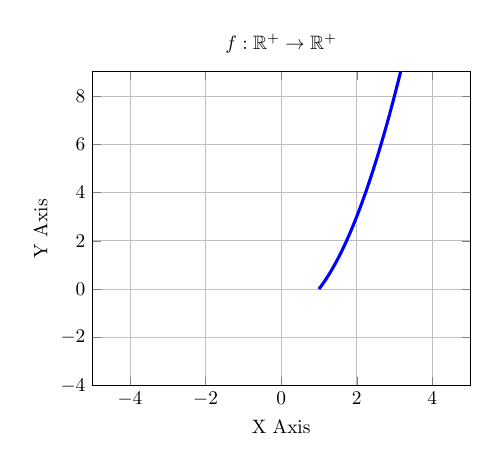
\begin{tikzpicture}[scale=0.7]
            \begin{axis}[
                xmax=5,
                xmin=-5,
                ymax=9,
                ymin=-4,
                samples=50,
                grid=major,
                xlabel={X Axis},
                ylabel={Y Axis},
                title={$f:\mathbb{R}^+\rightarrow\mathbb{R}^+$}
            ]
            \addplot[blue,ultra thick,domain=1:5](x,x^2-1);
        \end{axis}
        \end{tikzpicture}
        \label{sketch:exm-1}
    \end{subfigure}
    \hfill
    \begin{subfigure}[ht]{0.47\textwidth}
        \centering
        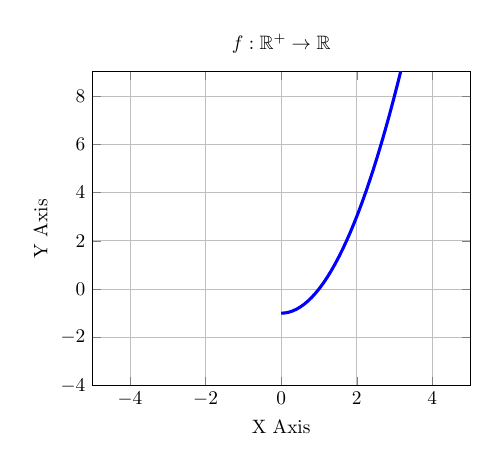
\begin{tikzpicture}[scale=0.7]
            \begin{axis}[
                xmax=5,
                xmin=-5,
                ymax=9,
                ymin=-4,
                samples=50,
                grid=major,
                xlabel={X Axis},
                ylabel={Y Axis},
                title={$f:\mathbb{R}^+\rightarrow\mathbb{R}$}
            ]
            \addplot[blue,ultra thick,domain=0:5](x,x^2-1);
        \end{axis}
        \end{tikzpicture}
        \label{sketch:exm-2}
    \end{subfigure}
    \vfill
    \begin{subfigure}[ht]{0.47\textwidth}
        \centering
        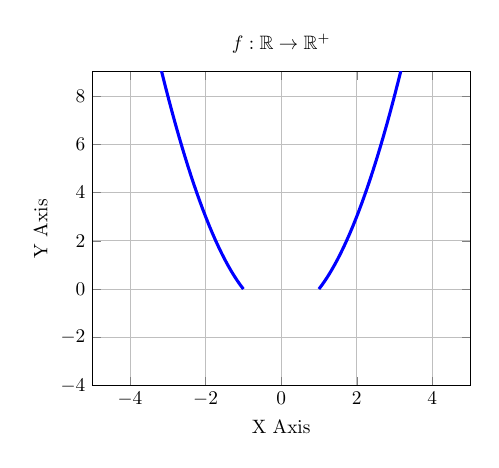
\begin{tikzpicture}[scale=0.7]
            \begin{axis}[
                xmax=5,
                xmin=-5,
                ymax=9,
                ymin=-4,
                samples=50,
                grid=major,
                xlabel={X Axis},
                ylabel={Y Axis},
                title={$f:\mathbb{R}\rightarrow\mathbb{R}^+$}
            ]
            \addplot[blue,ultra thick,domain=-5:-1](x,x^2-1);
            \addplot[blue,ultra thick,domain=1:5](x,x^2-1);
        \end{axis}
        \end{tikzpicture}
        \label{sketch:exm-3}
    \end{subfigure}
    \hfill
    \begin{subfigure}[ht]{0.47\textwidth}
        \centering
        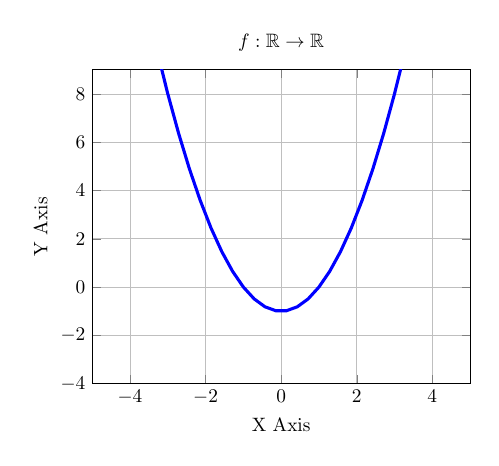
\begin{tikzpicture}[scale=0.7]
            \begin{axis}[
                xmax=5,
                xmin=-5,
                ymax=9,
                ymin=-4,
                samples=50,
                grid=major,
                xlabel={X Axis},
                ylabel={Y Axis},
                title={$f:\mathbb{R}\rightarrow\mathbb{R}$}
            ]
            \addplot[blue, ultra thick,domain=-5:9](x,x^2-1);
        \end{axis}
        \end{tikzpicture}
        \label{sketch:exm-4}
    \end{subfigure}
\end{figure}


% === End Section Includes ====

\newpage

\medskip
\printbibliography

\end{document}
